% Bioinformatics Original Paper, OUP authoring template (oup-authoring-template.cls, CTAN).
% Build: cd paper && tectonic main.tex
% Numbers come from results/a1/*.tsv (see the comment next to each table); do not edit them by hand.
% Items marked TODO are pending (software release, author block, supplementary file).
\documentclass[webpdf,contemporary,large]{oup-authoring-template}

\usepackage{booktabs}
\usepackage{tikz}
\usetikzlibrary{arrows.meta,positioning}
\newcommand{\todo}[1]{\textcolor{red}{[TODO: #1]}}

\journaltitle{Bioinformatics}
\DOI{DOI HERE}
\copyrightyear{2026}
\pubyear{2026}
\access{Advance Access Publication Date: Day Month Year}
\appnotes{Original Paper}

\begin{document}

\title[Label-efficient proxy-track selection]{Which of a thousand tracks should stand in for my cell type?
Label-efficient Bayesian discrimination of genomic foundation-model outputs}

\author[1,$\ast$]{\todo{First Author}}
\author[1]{\todo{Co-author}}
\authormark{\todo{Author} et al.}
\address[1]{\orgdiv{\todo{Department}}, \orgname{\todo{Institution}}, \orgaddress{\country{\todo{Country}}}}
\corresp[$\ast$]{Corresponding author. \todo{email}}

\received{Date}{0}{Year}
\revised{Date}{0}{Year}
\accepted{Date}{0}{Year}

\abstract{
\textbf{Motivation:} Sequence-to-function foundation models such as AlphaGenome predict the effect of any variant on
thousands of functional tracks, but a laboratory studying a particular cell type must still decide which track to
trust. Matching tracks by cell-type name is unreliable, and many cell types are not profiled at all. A few variants
can be measured, for example with a reporter assay, but it is unclear which variants to measure and how to turn a
handful of measurements into a choice among about a thousand highly correlated tracks.\\
\textbf{Results:} Each track is a hypothesis that the measured effect is an unknown affine function of its prediction.
We integrate out the calibration, form a posterior over tracks, keep metadata-matched tracks as the prior default, and
measure next the variant on which the tracks disagree most. In two pre-registered tests on saturation mutagenesis
reporter assays, eight chosen measurements beat eight random ones by 0.084 in Spearman correlation on 11 held-out
Kircher et al. regions with the cell type hidden ($P = 0.0024$). On 125 new Siraj et al. loci, all four
pre-registered hypotheses held. Where matched tracks existed, eight measurements did not harm them (mean $+0.010$;
3/125 loci worse by more than 0.05). Without them, eight measurements improved on the all-track mean by 0.048
($P = 8\times10^{-13}$). With only related-cell tracks, sixteen improved on those tracks' mean by 0.041. With random
measurements, the same inference fell below the label-free mean. Re-fitting the matched tracks to the few labels
lowered accuracy at all 125 loci. All four hypotheses still held when each locus was scored by a model checkpoint
that had not been trained on its region.\\
\textbf{Availability and implementation:} Code, pre-registrations and derived results are at
\url{https://github.com/ydvislab/AuraGenome-V} under the MIT licence. \todo{Zenodo archive DOI of the submitted
version, package name}\\
\textbf{Contact:} \todo{email}\\
\textbf{Supplementary information:} Supplementary data are available at \textit{Bioinformatics} online.}

\keywords{variant effect prediction, foundation models, active model selection, Bayesian experimental design,
massively parallel reporter assays}

\maketitle

%===============================================================================
\section{Introduction}

Deep sequence-to-function models predict the regulatory consequences of non-coding variants from DNA sequence alone
\citep{zhou2015deepsea,avsec2021enformer,linder2025borzoi}. The most recent of them, AlphaGenome, outputs thousands of
genome tracks for hundreds of human cell types and tissues, and scores any single-nucleotide variant on all of them
\citep{avsec2026alphagenome}. These predictions are accurate in aggregate. On the Kircher et al. saturation
mutagenesis data \citep{kircher2019saturation}, used in the CAGI5 challenge \citep{shigaki2019cagi5}, AlphaGenome is
among the best available predictors. Accuracy at a single locus is less certain, and performance on personal
expression variation is known to be weak \citep{sasse2023benchmarking,huang2023personal}.

A practical question sits between the model and the bench: \emph{which output track should a laboratory use for its
cell type?} The usual answer is to pick tracks whose biosample name matches the cell line in which the variants will
be studied. We found this unreliable. Across the 1,018 CAGE, DNase and ATAC tracks AlphaGenome predicts, the
name-matched track ranked between first and 27th by agreement with the measured effects in our development elements.
Choosing a different track changed the conclusions. At the \textit{PKLR} promoter in K562 cells, replacing K562 tracks
by HepG2 tracks lowered the directional accuracy on significant variants from 0.96 to 0.69--0.85, and the two sets of
tracks disagreed in sign on 13--32\% of significant variants. Many cell types used in the laboratory, including
patient-derived lines, are not profiled at all, and then there is no name to match.

Laboratories can, however, measure a few variants. Reporter assays, base editing or targeted allelic assays can
cheaply test a panel of perhaps 8--16 variants before a larger study. This turns proxy choice into a
label-efficient model selection problem: choose which variants to measure so that the measurements identify the track,
or the mixture of tracks, that best predicts the rest. Two features make it different from standard active model
selection \citep{karimi2021modelpicker,okanovic2025modelselector,kay2025coda}. First, the candidates are regression
outputs on arbitrary scales, so each track must be calibrated to the assay with an unknown slope and offset that a
handful of labels cannot pin down. Second, the candidates are a thousand strongly correlated heads of one network, not
a set of independently trained models.

We make three contributions.
(i) A Bayesian formulation in which each track is a hypothesis with an affine calibration that is integrated out in
closed form. The result is a posterior over tracks and a posterior-weighted prediction for unmeasured variants. A
metadata anchor prior makes the method safe when matched tracks exist.
(ii) A sequential design that measures the variant on which the posterior-weighted tracks disagree most, in the
tradition of model discrimination \citep{box1967discrimination}, applied here to about a thousand candidates.
(iii) Two pre-registered evaluations on independent saturation mutagenesis data (Kircher et al., 11 held-out regions;
Siraj et al., 125 new loci), plus a check of the dependence on the model's training exposure. These show when a few
measurements help, when they do not, and that the obvious alternative, re-fitting the matched tracks to the same few
labels, is harmful.

%===============================================================================
\section{Methods}

\begin{figure*}[t]
\centering
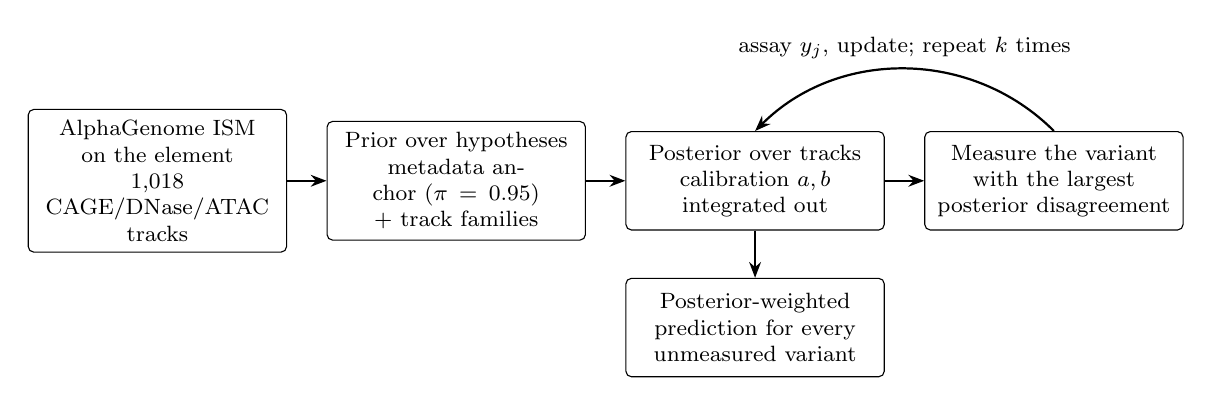
\begin{tikzpicture}[node distance=0.55cm and 0.5cm, every node/.style={font=\footnotesize},
  box/.style={draw, rounded corners=2pt, align=center, inner sep=4pt, text width=3.0cm, minimum height=1.25cm},
  arr/.style={-{Stealth[length=2mm]}, thick}]
\node[box] (tracks) {AlphaGenome ISM on the element\\ 1,018 CAGE/DNase/ATAC tracks};
\node[box, right=of tracks] (prior) {Prior over hypotheses\\ metadata anchor ($\pi=0.95$)\\ + track families};
\node[box, right=of prior] (post) {Posterior over tracks\\ calibration $a, b$\\ integrated out};
\node[box, right=of post] (pick) {Measure the variant with the largest posterior disagreement};
\node[box, below=0.6cm of post] (out) {Posterior-weighted prediction for every unmeasured variant};
\draw[arr] (tracks) -- (prior);
\draw[arr] (prior) -- (post);
\draw[arr] (post) -- (pick);
\draw[arr] (pick.north) to[out=135, in=45] node[above, align=center] {assay $y_j$, update; repeat $k$ times} (post.north);
\draw[arr] (post.south) -- (out.north);
\end{tikzpicture}
\caption{Overview. Each AlphaGenome track is a hypothesis that the measured effect is an affine function of the
track's predicted effect. With $k$ measured variants, the method updates a posterior over hypotheses whose prior keeps
the metadata-matched tracks as the default. It picks each next variant where the hypotheses disagree most and
reports a posterior-weighted prediction.}
\label{fig:overview}
\end{figure*}

\subsection{Problem}

A regulatory element is studied in cell type $c$. Saturation mutagenesis gives a set $V$ of single-nucleotide
variants with measured effects $y_j$; we pretend that only $k$ of them may be measured. For every variant, the
foundation model gives a predicted effect $x_{t,j}$ on each of $T$ tracks (here $T=1{,}018$). We want a prediction
$\hat y_j$ for every unmeasured variant, and the measurement panel $S \subset V$, $|S| = k$, that makes these predictions
as accurate as possible. Accuracy is the Spearman correlation between $\hat y$ and $y$ on variants not available for
measurement.

\subsection{Tracks as calibrated hypotheses}

For each track we use the standardised prediction $z_{t,j} = x_{t,j}/\mathrm{sd}_j(x_{t,\cdot})$. It is scaled over the
element but not centred, so the sign keeps the direction of the alternative allele. Hypothesis $t$ states
\begin{equation}
\begin{aligned}
y_j &= a + b\,z_{t,j} + \varepsilon_j,\\
a &\sim N(0,\alpha s^2),\quad b \sim N(0,\beta s^2),\quad \varepsilon_j \sim N(0,(1-\beta)s^2),
\end{aligned}
\end{equation}
where $s^2$ is the mean of $y_S^2$. Integrating out $a$ and $b$ gives the marginal likelihood of the measured panel,
\begin{equation}
y_S \mid t \sim N\!\left(0,\ s^2\left[(1-\beta)I + \alpha \mathbf{1}\mathbf{1}^\top + \beta z_{t,S} z_{t,S}^\top\right]\right),
\end{equation}
and the posterior $p(t \mid y_S) \propto p(t)\,p(y_S \mid t)$. The predictive mean of an unmeasured variant under $t$,
$m_{t,j} = E[y_j \mid t, y_S]$, follows from the Gaussian conditional. The reported prediction is the Bayesian model
average $\hat y_j = \sum_t p(t\mid y_S)\, m_{t,j}$ \citep{hoeting1999bma}. We fixed $\alpha = 0.1$ and $\beta = 0.5$
before any evaluation and did not tune them.

\subsection{Metadata anchor and track families}

When the model profiles the element's cell type, the mean of the metadata-matched tracks is a strong default. We add
it as one extra hypothesis, the \emph{anchor}, holding prior mass $\pi$. Its slope prior is centred on a positive
value, $b \sim N(\sqrt{\beta}\,s,\ (\beta/4)\,s^2)$, so that a negative slope has prior probability of about 2\%. Single
tracks share the remaining $1-\pi$. To prevent near-duplicate tracks from dominating the prior, we cluster tracks by
the correlation of their predictions (average linkage, $r \ge 0.9$; no labels used). The prior is split equally between
clusters and then within them, so duplicating a track changes nothing. When no matched tracks exist, there is no
anchor, and the method reduces to the track posterior with the family prior. The case $\pi = 0$ with a uniform prior is
the version we pre-registered first (v1). The anchor version (v2, $\pi = 0.95$) was chosen on development elements
only, frozen, and then tested (Section~\ref{sec:eval}).

\subsection{Choosing which variants to measure}

The panel is built sequentially from a pool of variants that could be measured. Given the current posterior, the next
variant maximises the posterior-weighted variance of the hypotheses' predictive means, $\mathrm{Var}_{t \sim p(t\mid
y_S)}[m_{t,j}]$, divided by the expected residual variance of that variant. This is the classical criterion for
discriminating between models \citep{box1967discrimination}, a member of the family of Bayesian experimental designs
\citep{rainforth2024modern}. We call this panel \emph{disc}. All panels are scored with the same inference, so panels
differ only in which variants are measured.

\subsection{Baselines}

\emph{Other panels.} We compare disc with random variants; the variants with the largest predicted effect under the
all-track mean, a common practical choice; and the variants with the largest unweighted disagreement across tracks.
\emph{Label-free references.} These are the mean of all tracks; the mean of the metadata-matched tracks; and, when
those are hidden, the mean of related-cell tracks. The best single track, chosen with all labels, is reported as a
reference, not an upper bound. \emph{Few-label regression.} Ridge regression and LASSO \citep{tibshirani1996lasso} over
all tracks, with the penalty chosen by leave-one-out on the same $k$ labels. This is the protocol used for AlphaGenome
on this benchmark, which there uses the full challenge training set. \emph{Same-budget metadata controls.} We include
\texttt{matched\_cal}, an affine re-fit of the matched mean with the $k$ labels, and \texttt{meta\_ridge}, which
calibrates the matched mean with a positive-slope prior and then fits ridge regression on the residuals over all
tracks.

\subsection{Data}

\textbf{Kircher et al.} \citep{kircher2019saturation} measured every possible substitution in 20 disease-associated
regulatory elements by saturation mutagenesis MPRA. We used the 22 experiments measured in human cells (27,789
variants, 561--1,800 per experiment). Five experiments from five regions (\textit{PKLR}, \textit{F9},
\textit{HNF4A}, \textit{IRF6}, \textit{BCL11A}) formed the development set. The other 17 experiments from 11 regions
formed the test set; several of them were measured in cell lines AlphaGenome does not profile (for example
SK-MEL-28 and glioblastoma lines).
\textbf{Siraj et al.} \citep{siraj2026functional,siraj2025data} measured all substitutions in 200-bp oligonucleotides
around fine-mapped trait variants, in K562 and HepG2 cells. Of the 128 published elements, we used the reference
background of 125. One was excluded because its reference background contains a deletion, and two because the oligo
had no unique exact match in GRCh38. This left 74,975 substitutions, each measured in both cell types; the effect is
the reported log$_2$ allelic skew.
\textbf{Predictions.} We scored every variant by in-silico mutagenesis with AlphaGenome (API, 1-Mb context) on all
CAGE, DNase and ATAC tracks for human biosamples \citep{avsec2026alphagenome}. These assays derive from ENCODE and
FANTOM5 \citep{encode2020expanded,fantom2014atlas}. The main analyses use the default distilled checkpoint
(ALL\_FOLDS).

\textbf{Training data, test sets and homology.} The method trains no model. AlphaGenome is used frozen, and the only
labels are the $k$ measured variants of the element being predicted. No measured effect from any other element, and no
evaluation variant, enters the inference. Performance is reported on two independent test sets defined before analysis:
11 Kircher regions not used during development, and 125 Siraj loci not used at any stage of method design. No test
region overlaps a development region; the nearest pair, one Siraj locus within 500 kb of the \textit{IRF6} development
element, shares only long-range model context. Two kinds of exposure remain. MPRA labels were never part of
AlphaGenome's training, but its training tracks cover these genomic regions. We test the dependence on this exposure
with checkpoints that held out the genomic fold of each locus (Section~\ref{sec:c1}). The folds are the model developers' split of the genome into
sets of intervals \todo{state from the AlphaGenome/Borzoi split description how homologous sequence is assigned to
folds; not yet verified}.
Leave-one-out is not used for evaluation. It appears only inside the ridge and LASSO baselines, to choose a penalty
from the $k$ labels, and in a leave-one-element-out sensitivity check of $\pi$ on the development set.

\subsection{Evaluation protocol and pre-registration}
\label{sec:eval}

In each of 200 repeats (seed 0), half of an element's variants form the pool that could be measured. Panels are built
from the pool, and every method and reference is scored by Spearman correlation on the same variants outside the pool.
Experiments that share a genomic region are averaged, and the analysis unit is the region (Kircher) or the locus
(Siraj; its two cell types are averaged).
We simulate three situations by hiding tracks. In C1 all tracks are kept. In C2 only the element's own cell line is
hidden, and related-cell tracks remain. In C3 both are hidden, which approximates a cell type the model does not
profile. Related cell types were listed from track metadata before any result was seen.
Two pre-registrations were committed together with frozen code before the test data were analysed.
\emph{Kircher test (v1):} H1, disc beats random panels (one-sided Wilcoxon, $P<0.05$); H2, disc beats the
all-track mean by at least 0.03 in at least 7/11 regions; H3 (secondary), disc beats high-predicted-effect panels.
\emph{Siraj test (frozen v2):} P1, non-inferiority to the matched mean in C1 at $k=8$ (one-sided 95\% bootstrap lower
bound above $-0.02$); P2, at most 15\% of loci worse by more than 0.05 (one-sided 95\% Clopper--Pearson upper bound);
P3, improvement over the all-track mean in C3 at $k=8$ of at least 0.03 with $P<0.05$; P4, improvement over the
related-cell mean in C2 at $k=16$ with $P<0.05$. The safety-net claim required P1, P2 and either P3 or P4.
Analyses added after the pre-registrations are labelled as such.

%===============================================================================
\section{Results}

\subsection{A few chosen measurements recover the proxy when the cell type is hidden}

On the Kircher test regions with the element's own and related cell types hidden (C3), eight disc measurements gave a
mean Spearman correlation of 0.370, against 0.286 for eight random measurements and 0.296 for the label-free all-track
mean (Table~\ref{tab:kircher}, Fig.~\ref{fig:curve}). The pre-registered H1 held: disc beat random panels by 0.084,
9/11 regions, $P = 0.0024$. H2 also held: disc beat the all-track mean by 0.074, 8/11 regions. H3 did not: the margin
over high-predicted-effect panels was 0.031, $P = 0.18$.
The gains were concentrated in elements with signal and room above the average. They included \textit{HBG1}, where
the posterior-weighted prediction exceeded the best single track, and \textit{IRF4} in SK-MEL-28, a cell line the
model does not profile. Elements with very few significant variants (\textit{FOXE1}, 5; one \textit{MYC} enhancer,
11) or with an all-track mean already near the best track (\textit{TERT}) showed no gain.

With the same eight labels, regression over all tracks was much worse (post hoc). Disc beat random panels with LASSO
by 0.110--0.182, depending on how all-zero LASSO fits are treated ($P \le 0.0024$), and random panels with ridge by
0.116. On the disc panel itself, the Bayesian track posterior still beat LASSO by 0.034--0.048 and ridge by 0.023
($P = 0.042$). So both the panel and the inference contribute.

\begin{table*}[t]
\centering
% results/a1/common_eval_test_k8_by_element.tsv (region means), common_eval_test_decision.txt,
% common_eval_regression_baselines_k8.tsv
\caption{Kircher test set, C3 (own and related cell types hidden), $k=8$, 11 regions. Spearman correlation on the
common evaluation set. $^\dagger$Added after pre-registration (first 50 repeats); for LASSO the range covers three
rules for all-zero fits.}
\label{tab:kircher}
\begin{tabular}{llccc}
\toprule
Panel & Prediction & Mean $\rho$ & Ours $-$ this row & Regions $>0$, one-sided $P$ \\
\midrule
disc & track posterior (ours) & 0.370 & --- & --- \\
random & track posterior & 0.286 & $+0.084$ & 9/11, 0.0024 \\
high predicted effect & track posterior & 0.338 & $+0.031$ & --, 0.18 \\
static disagreement & track posterior & 0.361 & $+0.009$ & --, -- \\
none & all-track mean & 0.296 & $+0.074$ & 8/11, -- \\
random & LASSO$^\dagger$ & -- & $+0.110$ to $+0.182$ & 9--10/11, $\le$0.0024 \\
random & ridge$^\dagger$ & -- & $+0.116$ & 8/11, 0.0068 \\
disc & LASSO$^\dagger$ & -- & $+0.034$ to $+0.048$ & 8/11, $\le$0.016 \\
disc & ridge$^\dagger$ & -- & $+0.023$ & 8/11, 0.042 \\
all labels & best single track (reference) & 0.454 & --- & --- \\
\bottomrule
\end{tabular}
\end{table*}

\begin{figure}[t]
\centering
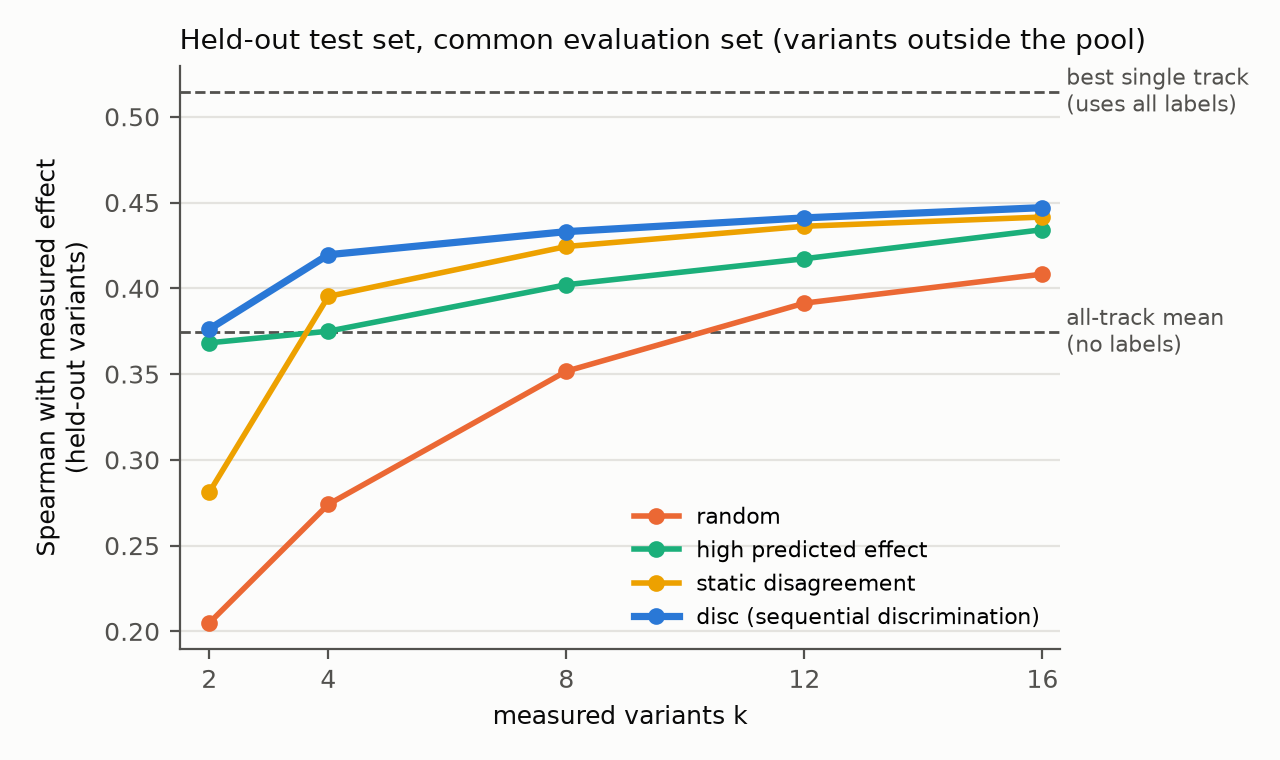
\includegraphics[width=\linewidth]{figures/fig5_test_learning_curve_common_eval.png}
\caption{Kircher test set (C3): Spearman correlation on held-out variants against the number of measured variants
$k$. All panels use the same track posterior. Dashed lines are the label-free all-track mean and the best single track
chosen with all labels (a reference).}
\label{fig:curve}
\end{figure}

\subsection{When matched tracks exist, the prior must default to them}

The C3 setting is a stress test. In practice, a laboratory working in a profiled cell type would simply use the
matched tracks. When we kept all tracks (C1), the anchor-free method (v1) was on average 0.029 below the label-free
matched mean at $k=8$, and 7/11 regions were worse by more than 0.05 (post hoc; Table~\ref{tab:v2}). It helped only
where the matched tracks were poor (\textit{LDLR}: matched mean 0.24, v1 0.51). It lost where they were good
(\textit{SORT1}: 0.65 against 0.48).

The metadata anchor removed most of this harm. With $\pi = 0.95$, chosen on the development set by a rule fixed in
advance (and re-chosen in 4/5 leave-one-element-out runs), v2 was level with the matched mean at $k=8$ ($+0.001$,
1/11 harmed) and ahead at $k=16$ ($+0.018$, none harmed). Rescue was slower: at \textit{LDLR}, v2 reached 0.29 at
$k=8$ and 0.41 at $k=16$. On the same disc panel, v2 and the simpler \texttt{meta\_ridge} control were tied on
Kircher. Re-fitting the matched mean with eight labels (\texttt{matched\_cal}) was harmful, because the fitted slope
can flip sign (\textit{LDLR} fell to 0.14).

\begin{table}[t]
\centering
% results/a1/v2_test_configs.tsv
\caption{Kircher test set, C1 (all tracks kept), 11 regions. Difference from the label-free matched-track mean
(0.405); harmed = regions worse by more than 0.05. v1 and the controls were analysed after the v1 pre-registration;
v2 was frozen on the development set before this run.}
\label{tab:v2}
\begin{tabular}{lcccc}
\toprule
& \multicolumn{2}{c}{$k=8$} & \multicolumn{2}{c}{$k=16$} \\
Method & diff. & harmed & diff. & harmed \\
\midrule
v1 (no anchor) & $-0.029$ & 7 & $-0.014$ & 4 \\
v2 (anchor, frozen) & $+0.001$ & 1 & $+0.018$ & 0 \\
disc panel + \texttt{meta\_ridge} & $+0.002$ & -- & $+0.018$ & -- \\
random panel + \texttt{matched\_cal} & $-0.079$ & -- & $-0.043$ & -- \\
\bottomrule
\end{tabular}
\end{table}

\subsection{Pre-registered validation on 125 new loci}

We then ran the frozen v2 once on the Siraj et al. data (Table~\ref{tab:siraj}, Fig.~\ref{fig:siraj}). All four
primary hypotheses held. In C1, eight measurements did not harm the matched tracks. The mean difference was $+0.010$
with a one-sided lower bound of $+0.005$, against a margin of $-0.02$. Only 3/125 loci were worse by more than 0.05
(upper bound 6.1\%, against 15\%). At $k=16$ the difference was $+0.020$, and one locus was harmed. In C3, eight
measurements improved on the all-track mean by 0.048 (0.391 to 0.440; $P = 8\times10^{-13}$). In C2, sixteen
measurements improved on the related-cell mean by 0.041 (0.412 to 0.453; $P = 1\times10^{-19}$). The pre-registered
decision was therefore that the safety-net claim is supported.

The secondary analyses, which report effect sizes only, sharpen this picture. The panel matters most when there is no
anchor. In C3, disc beat random panels by 0.093 at 122/125 loci, and with random panels the same inference (0.346) fell
below the label-free mean (0.391). In C1, the advantage was 0.018. Unlike on Kircher, v2 was slightly ahead of
\texttt{meta\_ridge} on the same panel ($+0.008$, 97/125, two-sided $P<0.001$). Re-fitting the matched mean with eight
labels lowered accuracy at every one of the 125 loci (mean $-0.079$). The family prior had no effect ($-0.002$,
$P = 0.11$); we keep it only because it makes the method invariant to duplicated tracks. The C1 gain was larger in
HepG2 ($+0.017$) than in K562 ($+0.003$, interval including 0).

\begin{table*}[t]
\centering
% results/a1/siraj_decision.txt, siraj_secondary.tsv
\caption{Pre-registered Siraj test, frozen v2, 125 loci (two cell types averaged per locus). $D$ is the mean paired
difference in Spearman correlation.}
\label{tab:siraj}
\begin{tabular}{llcc}
\toprule
Hyp. & Comparison & $D$ & Criterion, result \\
\midrule
P1 & C1, $k=8$: v2 $-$ matched mean & $+0.010$ & LB $+0.005 > -0.02$, holds \\
P2 & C1, $k=8$: loci with $D<-0.05$ & 3/125 & UB $0.061 \le 0.15$, holds \\
P3 & C3, $k=8$: v2 $-$ all-track mean & $+0.048$ & $\ge 0.03$, $P=8\!\times\!10^{-13}$, holds \\
P4 & C2, $k=16$: v2 $-$ related mean & $+0.041$ & $>0$, $P=1\!\times\!10^{-19}$, holds \\
\midrule
S1 & C3, $k=8$: disc $-$ random panel & $+0.093$ & 122/125 $>0$ \\
S2 & C1, $k=8$: v2 $-$ \texttt{meta\_ridge} & $+0.008$ & 97/125 $>0$ \\
S3 & C1, $k=8$: \texttt{matched\_cal} $-$ matched & $-0.079$ & 0/125 $>0$ \\
S5 & C1, $k=8$: family $-$ uniform prior & $-0.002$ & $P=0.11$ \\
\bottomrule
\end{tabular}
\end{table*}

\begin{figure*}[t]
\centering
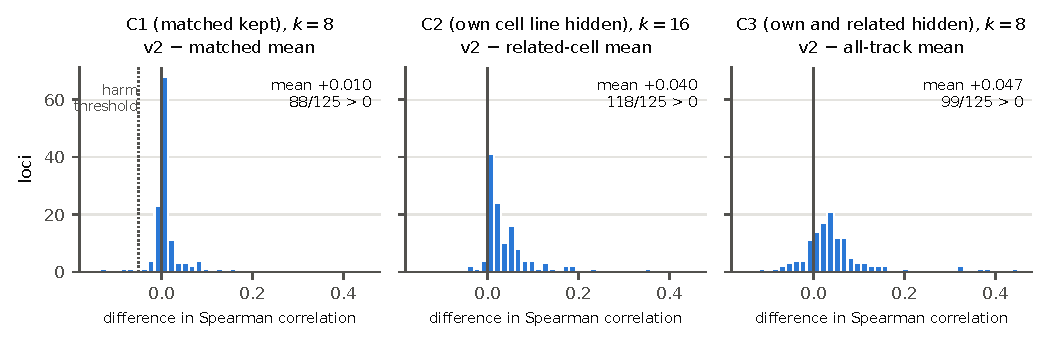
\includegraphics[width=\textwidth]{figures/fig_siraj.pdf}
\caption{Per-locus paired differences on the 125 Siraj loci for the three pre-registered primary comparisons. The
dotted line marks the pre-registered harm threshold ($-0.05$).}
\label{fig:siraj}
\end{figure*}

\subsection{Dependence on the model's training exposure}
\label{sec:c1}

The distilled ALL\_FOLDS checkpoint was trained on every genomic region, including those studied here. AlphaGenome
also provides four checkpoints, each trained without one fold of the genome. We reran the Kircher analysis with, for
each element, the checkpoint that never trained on its region. The specification and reading rule were committed
before the runs. All absolute accuracies fell by about 0.035; for example, the best single track fell from 0.465 to
0.428. The advantage over random panels became larger: $+0.093$, 10/11 regions, $P = 0.0015$. The advantage over the
all-track mean shrank to $+0.054$ (7/11, $P = 0.062$), mainly at \textit{IRF4}, \textit{MSMB} and \textit{LDLR}. The
difference between v2 and the matched mean moved from $+0.001$ to $-0.006$, with one harmed region in both cases. By
our pre-declared rule, which required every contrast to keep its sign, we report these conclusions as dependent on
training exposure. In hindsight, a sign rule is too strict for a non-inferiority quantity that is near zero.

Eleven regions give little power, so we repeated the check on the 125 Siraj loci. We used the thresholds of the
Siraj pre-registration and a reading rule committed before scoring. Each locus overlaps the training intervals of
exactly one fold, so each has a unique held-out checkpoint. Absolute accuracies fell again, by 0.04--0.07. The
matched-track mean fell from 0.474 to 0.402, v2 with eight labels from 0.483 to 0.426, and the best single track from
0.535 to 0.492. With matched and related tracks hidden, the all-track mean fell from 0.391 to 0.347 and v2 from 0.440 to
0.398. All four pre-registered hypotheses still held, with larger effects (Supplementary Table~\todo{S}). P1:
$+0.024$, one-sided lower bound $+0.017$, 1/125 loci harmed. P3: $+0.052$, $P = 3\times10^{-13}$. P4: $+0.054$,
$P = 7\times10^{-21}$. Paired over loci, the change from ALL\_FOLDS was $+0.015$ for P1 (95\% bootstrap interval
$+0.008$ to $+0.022$), $+0.014$ for P4 ($+0.006$ to $+0.021$) and $+0.003$ for P3 ($-0.006$ to $+0.013$). The matched
tracks lost the most accuracy without training exposure, and the measurements recovered part of that loss. On this
larger set, the advantage over the all-track mean did not weaken as it did on the 11 Kircher regions.

\subsection{One assay round is enough (post hoc)}
\label{sec:cmp}

After both tests we compared acquisition alternatives requested in review. All used the frozen v2 inference, the same
pools and 50 repeats per unit; the specification, and the rule that fixed the stopping threshold on the development
elements, were committed before the test runs. A one-round panel (\emph{batch}) runs disc's sequence without
measurements: each chosen variant's label is replaced by the current posterior-average prediction. At $k=8$, disc was
ahead of batch by only 0.002--0.005 on Siraj and 0.003--0.004 on Kircher; every 95\% interval lay within $\pm0.02$, our
pre-declared equivalence margin. Ranking variants once by prior disagreement was worse without an anchor (C3: disc
ahead by 0.021). Choosing by the expected information gain about which track is correct, with each track's calibration
uncertainty in its predictive variance, matched disc (differences $\le 0.003$). A stopping rule that halts once the
averaged prediction stops changing used about four labels with matched tracks and eight without, and matched fixed
eight-label panels ($-0.008$ to $+0.001$ on Siraj). It lost 0.014--0.027 against sixteen labels, however, and failed
our non-inferiority criterion in C2 and C3. On Siraj, disc beat largest-predicted-effect panels without an anchor (C3:
$+0.024$, 95\% interval $+0.018$ to $+0.031$, 97/125 loci) and tied them with matched tracks kept ($+0.007$).

%===============================================================================
\section{Discussion}

Foundation models now give laboratories a thousand candidate predictions for every variant. Our results suggest a
simple protocol for choosing among them. Start from the tracks whose metadata match the cell type. Measure about eight
variants chosen to split the competing tracks. Let the measurements move the prediction away from the default only
when they contradict it. On 125 new loci, this cost nothing on average when the default was available: the mean
difference was slightly positive, and 3/125 loci lost more than 0.05. It recovered 0.04--0.05 when the default was
missing or only approximate.

Three findings are, in our view, more general than the method. First, \emph{which} variants are measured matters as
much as how they are modelled. With random measurements, the same Bayesian inference was worse than not measuring at
all. Second, the obvious shortcut of re-fitting the matched track to the new measurements is harmful with eight
labels, because the slope is poorly determined and can flip. A prior centred on the metadata default avoids this.
Third, the output should be an \emph{average}. With matched tracks kept on Kircher at $k=8$, the posterior-weighted
prediction was ahead of the single most probable track by 0.045 for v1 and 0.007 for v2. At
\textit{HBG1} it even exceeded the best single track chosen with all labels. Reporting one proxy track therefore
discards information.

The method is closely related to label-efficient model selection for pretrained classifiers
\citep{karimi2021modelpicker,okanovic2025modelselector,kay2025coda,durmazkeser2025selectllm}. It differs in three
ways: candidates are regression outputs with an unknown per-candidate calibration, which we integrate out; the output
is a model average rather than a single selected model; and the candidates are about a thousand strongly correlated
heads of one network. Our acquisition rule is the classical discrimination criterion \citep{box1967discrimination}.
On Kircher its edge over simpler targeted panels was not significant (H3). On the larger Siraj set it beat
largest-predicted-effect panels when no anchor existed, but tied them when matched tracks were kept
(Section~\ref{sec:cmp}). Computing the information gain directly \citep{rainforth2024modern} did not help, and a panel
fixed before any measurement was nearly as good as sequential choice. A laboratory can therefore order the whole
panel at once.

\textbf{Limitations.} K562 and HepG2 are profiled by AlphaGenome. For Siraj, the situations without matched tracks are
simulated by hiding tracks, not observed in truly unprofiled cells. The evaluation is retrospective, and a prospective
panel may behave differently. Absolute correlations are moderate (0.44--0.49 on Siraj), and gains are small where the
assay has few significant variants. On Kircher, v2's anchor did not beat the simpler metadata-centred ridge; on Siraj
it was only slightly ahead. We have no stopping rule that matches sixteen labels; ours stopped too early. The checkpoint
analysis shows that training exposure inflates absolute accuracy by 0.04--0.07. On the 11 Kircher regions the
advantage over the label-free mean weakened on held-out folds; on the 125 Siraj loci it did not. Our held-out folds
are defined by the element's own window; the model's 1~Mb context still reaches sequence from other folds.

%===============================================================================
\section{Conclusion}

A handful of well-chosen measurements is enough to decide, among about a thousand foundation-model tracks, which to
trust for a cell type. This holds as long as the decision starts from the metadata default and the measurements are
chosen to discriminate. In two pre-registered tests, the approach was safe when matched tracks exist and improved
predictions when they do not, with eight to sixteen measured variants that can be chosen in a single round.

\section*{Acknowledgements}
\todo{acknowledgements}
\todo{Required by the journal's LLM policy, to be completed by the authors: declare where AI tools were used (for
example code, analysis scripts, figures, language editing), in this section or in Methods and in the cover letter.
The journal does not accept papers drafted with LLMs; the final text must be written by the authors.}

\section*{Author contributions}
\todo{CRediT roles for each author}

\section*{Funding}
\todo{funding}

\section*{Conflict of interest}
None declared.

\section*{Data availability}
Kircher et al. data are available from the original publication \citep{kircher2019saturation}
\todo{database accession}. Siraj et al.
saturation mutagenesis data are available from Zenodo under CC-BY-NC \citep{siraj2025data}; they are not
redistributed. AlphaGenome predictions can be regenerated with the public API and the scripts in the repository.
Pre-registrations, code and all derived tables are at \url{https://github.com/ydvislab/AuraGenome-V}.

\bibliographystyle{plainnat}
\bibliography{refs}

\end{document}
